\documentclass[12pt]{beamer}
\usepackage{algorithm2e} %pseudocodigos
\usepackage{algorithmic} %pseudocodigos
\usepackage{float}
\usetheme{Berkeley}



\usepackage{graphicx}
\graphicspath{{imagens/}}
\usepackage{booktabs}
\usepackage[english]{babel}



%\logo{\includegraphics[height=1cm]{example-image-c}}
%\logo{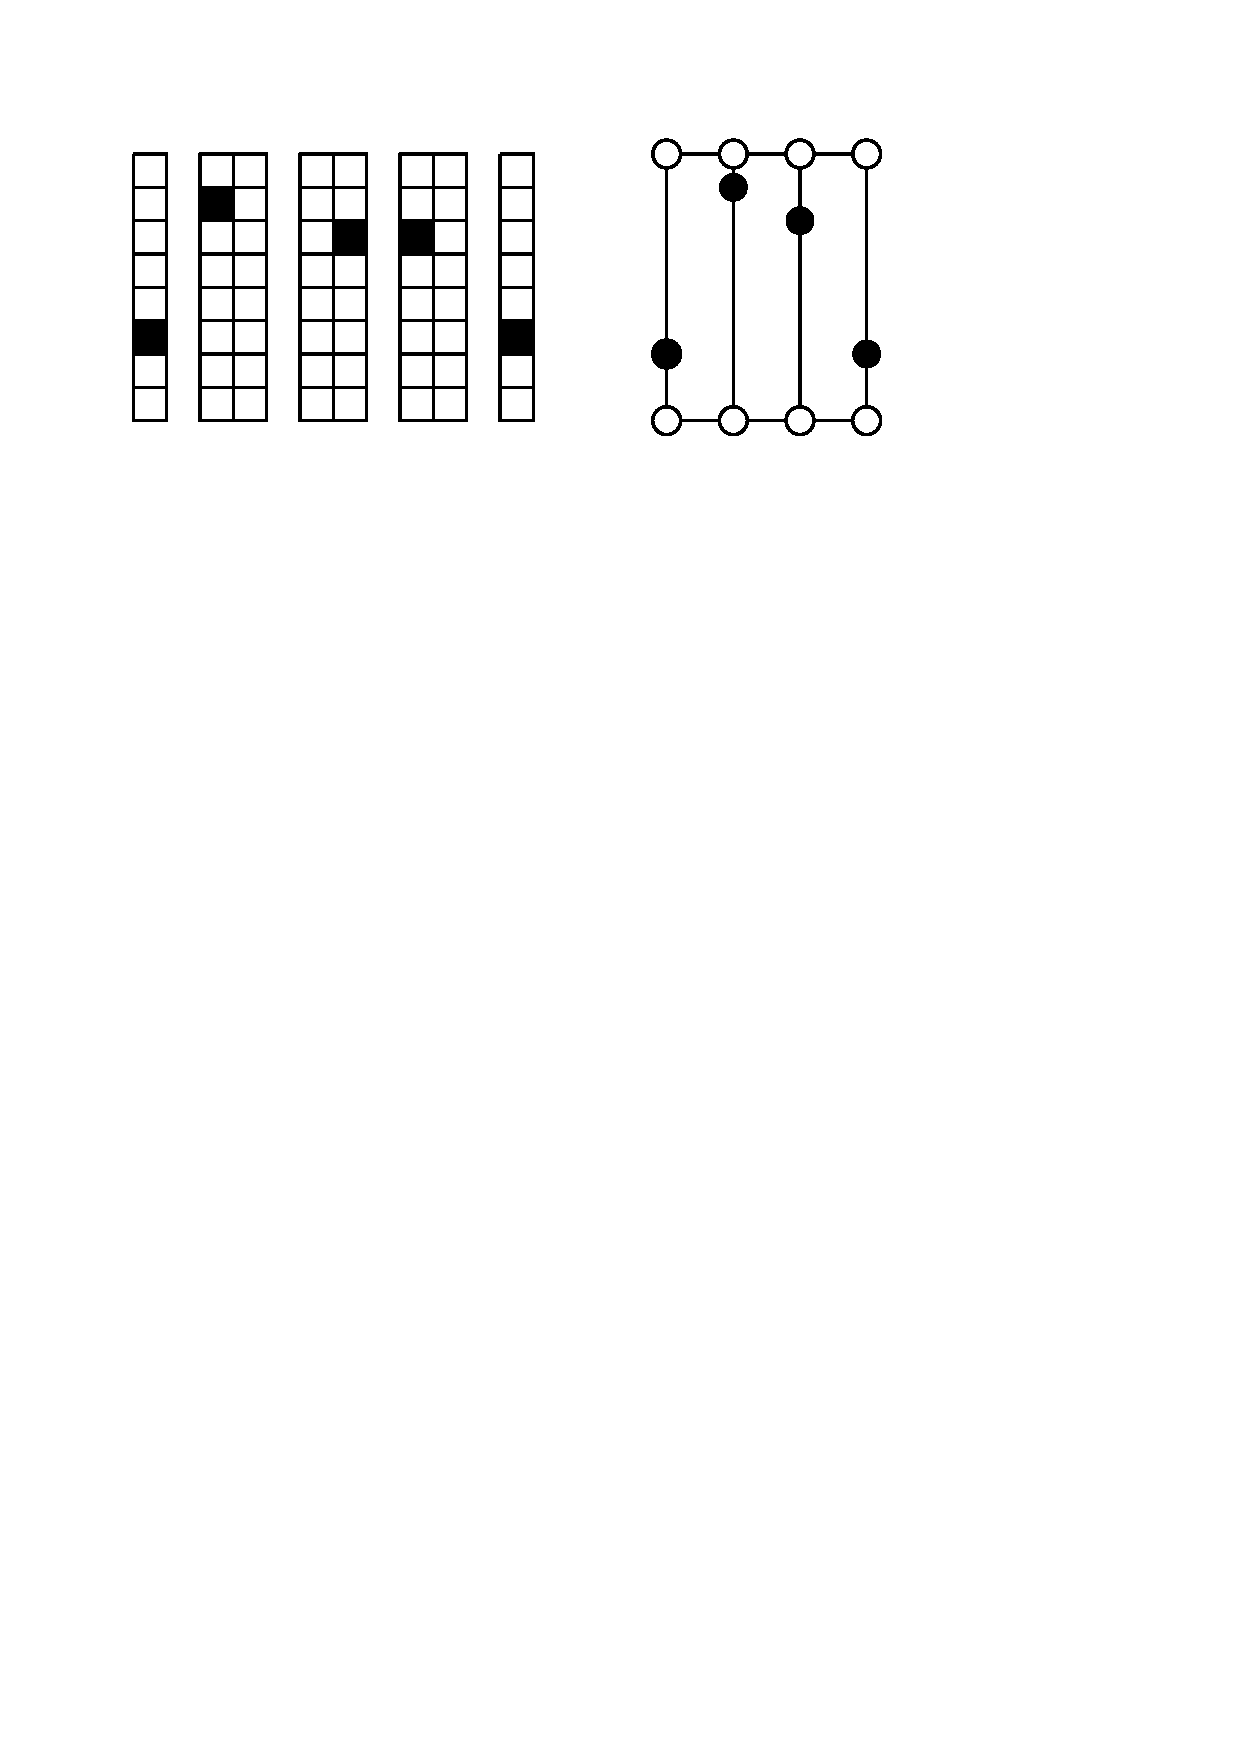
\includegraphics[height=1cm]{CD_1}}
\logo{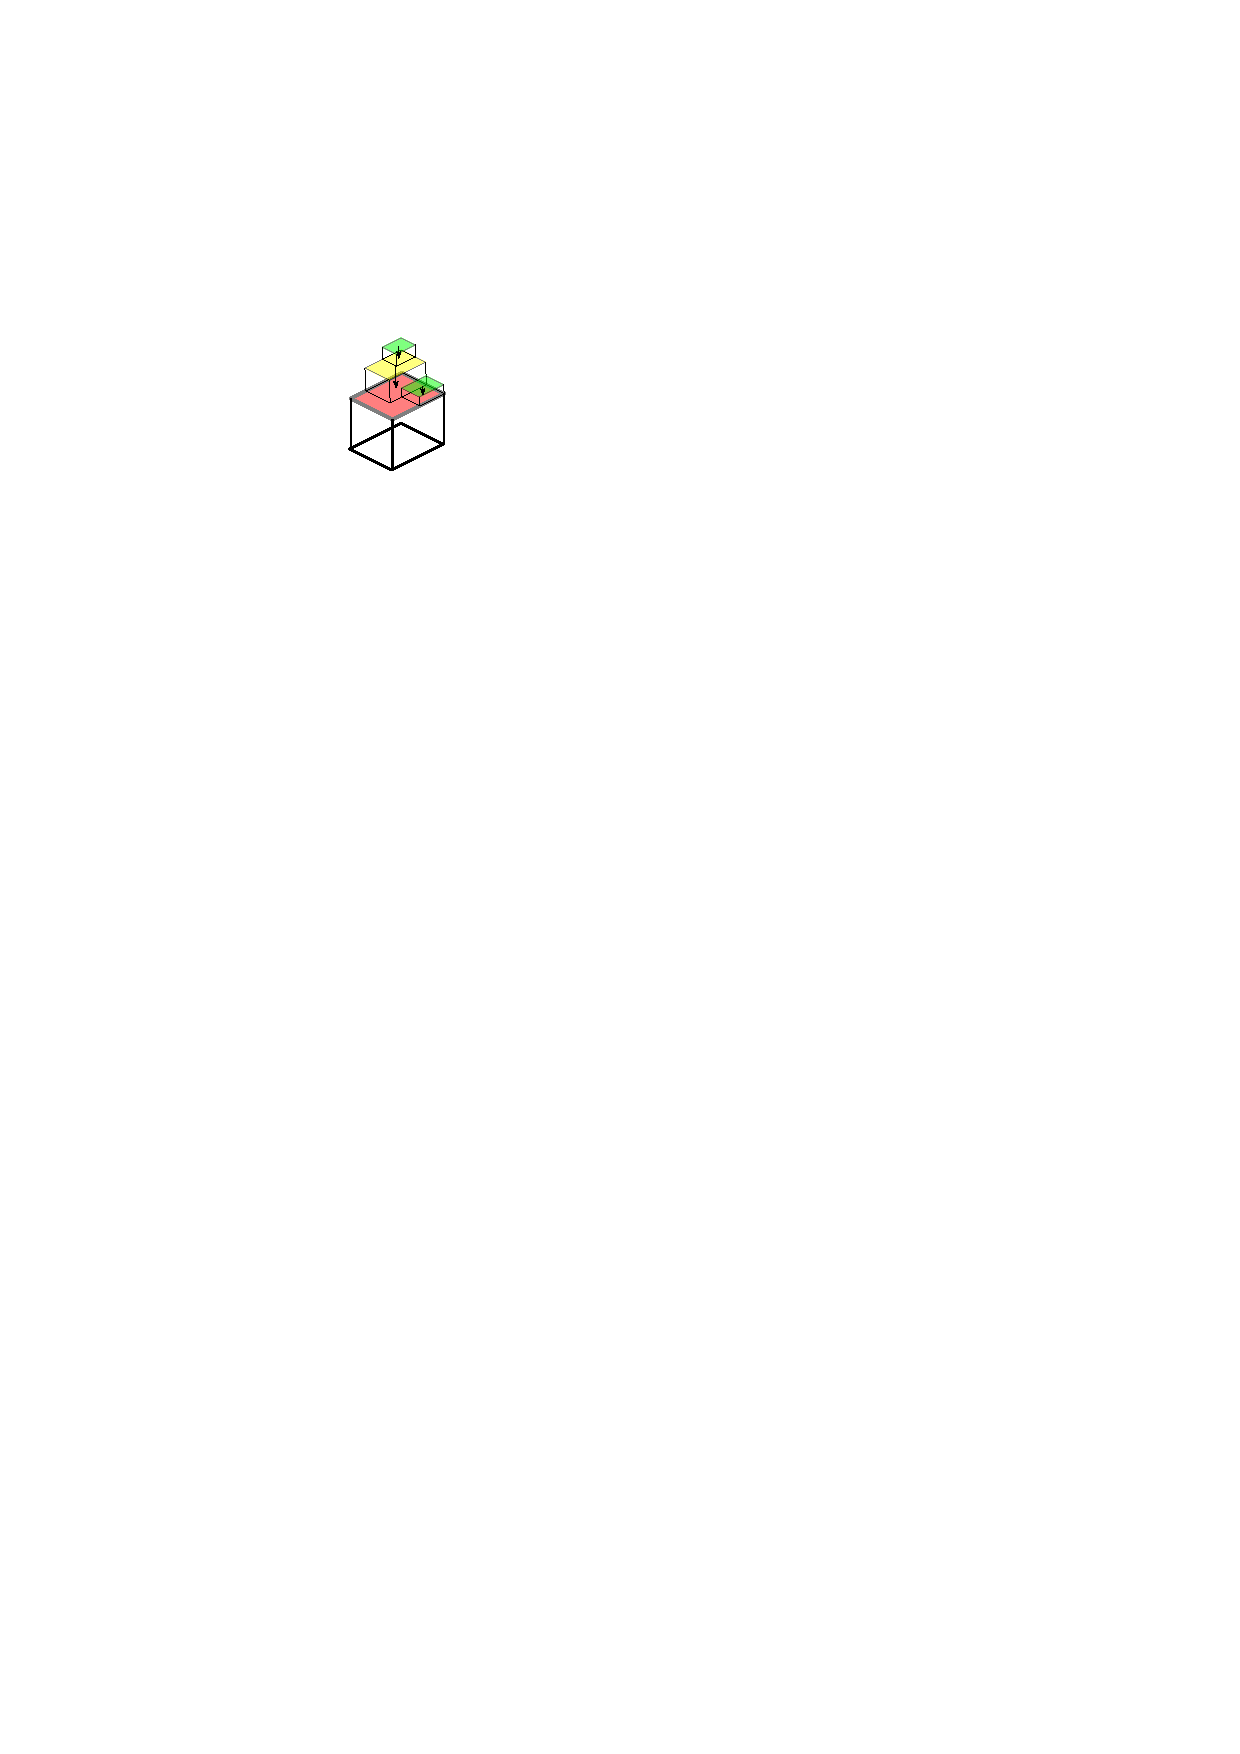
\includegraphics[width=0.1\linewidth]{pressao_caixas}}
\title[]{Uma nova heur\'istica para o "Single-Picker-Routing-Problem" com restri\c{c}\~oes pr\'aticas de carregamento}



\author{Alexandre Checoli Choueiri}
\institute[AI]
{UFPR  \\ % Your institution for the title page
	\medskip
	\textit{alexandrechecoli@gmail.com} % Your email address
	
}
\date{\today}

\begin{document}
	
	\begin{frame} 
		\titlepage % Print the title page as the first slide	
	\end{frame}
	
	\begin{frame}{Sum\'ario}
		\tableofcontents
	\end{frame}
		
	
\section{Motiva\c{c}\~ao}
%%%%%%%%%%%%%%%%%%%%%%%%%%%%%%%%%%%%%%%%%%%%%%%%%%%%%%%%%%%%%%%%%%%%%%%%%%%%%%%%%%
\begin{frame}{Motiva\c{c}\~ao}
	\begin{enumerate}
		\item {\bfseries Fidedignidade :}	
		Estudos na \'area de Roteamento em \'armazens carecem de Fidedignidade, ao considerarem somente aspectos relacionados \'a rota.
	\end{enumerate}
	\begin{enumerate}
		\item {\bfseries Depend\^encia de Solvers :}	
		Muitas das solu\c{c}\~oes tratadas na literatura dependem de Softwares comerciais para que os modelos sejam otimizados.
	\end{enumerate}	
\end{frame}

\section{Objetivos}
%%%%%%%%%%%%%%%%%%%%%%%%%%%%%%%%%%%%%%%%%%%%%%%%%%%%%%%%%%%%%%%%%%%%%%%%%%%%%%%%%%
\begin{frame}{Objetivos}

	\begin{itemize}
		\item{Estudar o modelo matematico de Scholz, adapatando-o para um m\'etodo heur\'istico}
		\pause	
		\item{A adapatar a Heur\'istica com restri\c{c}\~oes de carregamento:}
		\begin{itemize}
			\item{Estabilidade vertical}
			\item{Empilhamento m\'aximo} 
		\end{itemize}
		\pause
		\item{Respeitando a pol\'itica L.I.F.O para coleta dos itens}
	\end{itemize}
\end{frame}


	\begin{frame}{Descri\c{c}\~ao do problema}
%%%%%%%%%%%%%%%%%%%%%%%%%%%%%%%%%%%%%%%%%%%%%%%%%%%%%%%%%%%%%%%%%%%%%%%%%%%%%%%%%%
	\section{Descri\c{c}\~ao do problema (SPRP)}
	\framesubtitle{Original (SPRP)}	
		Definir a rota em em um armaz\'em,de tal forma a visitar todos os pontos de coleta:
			\begin{figure}
			\pause
			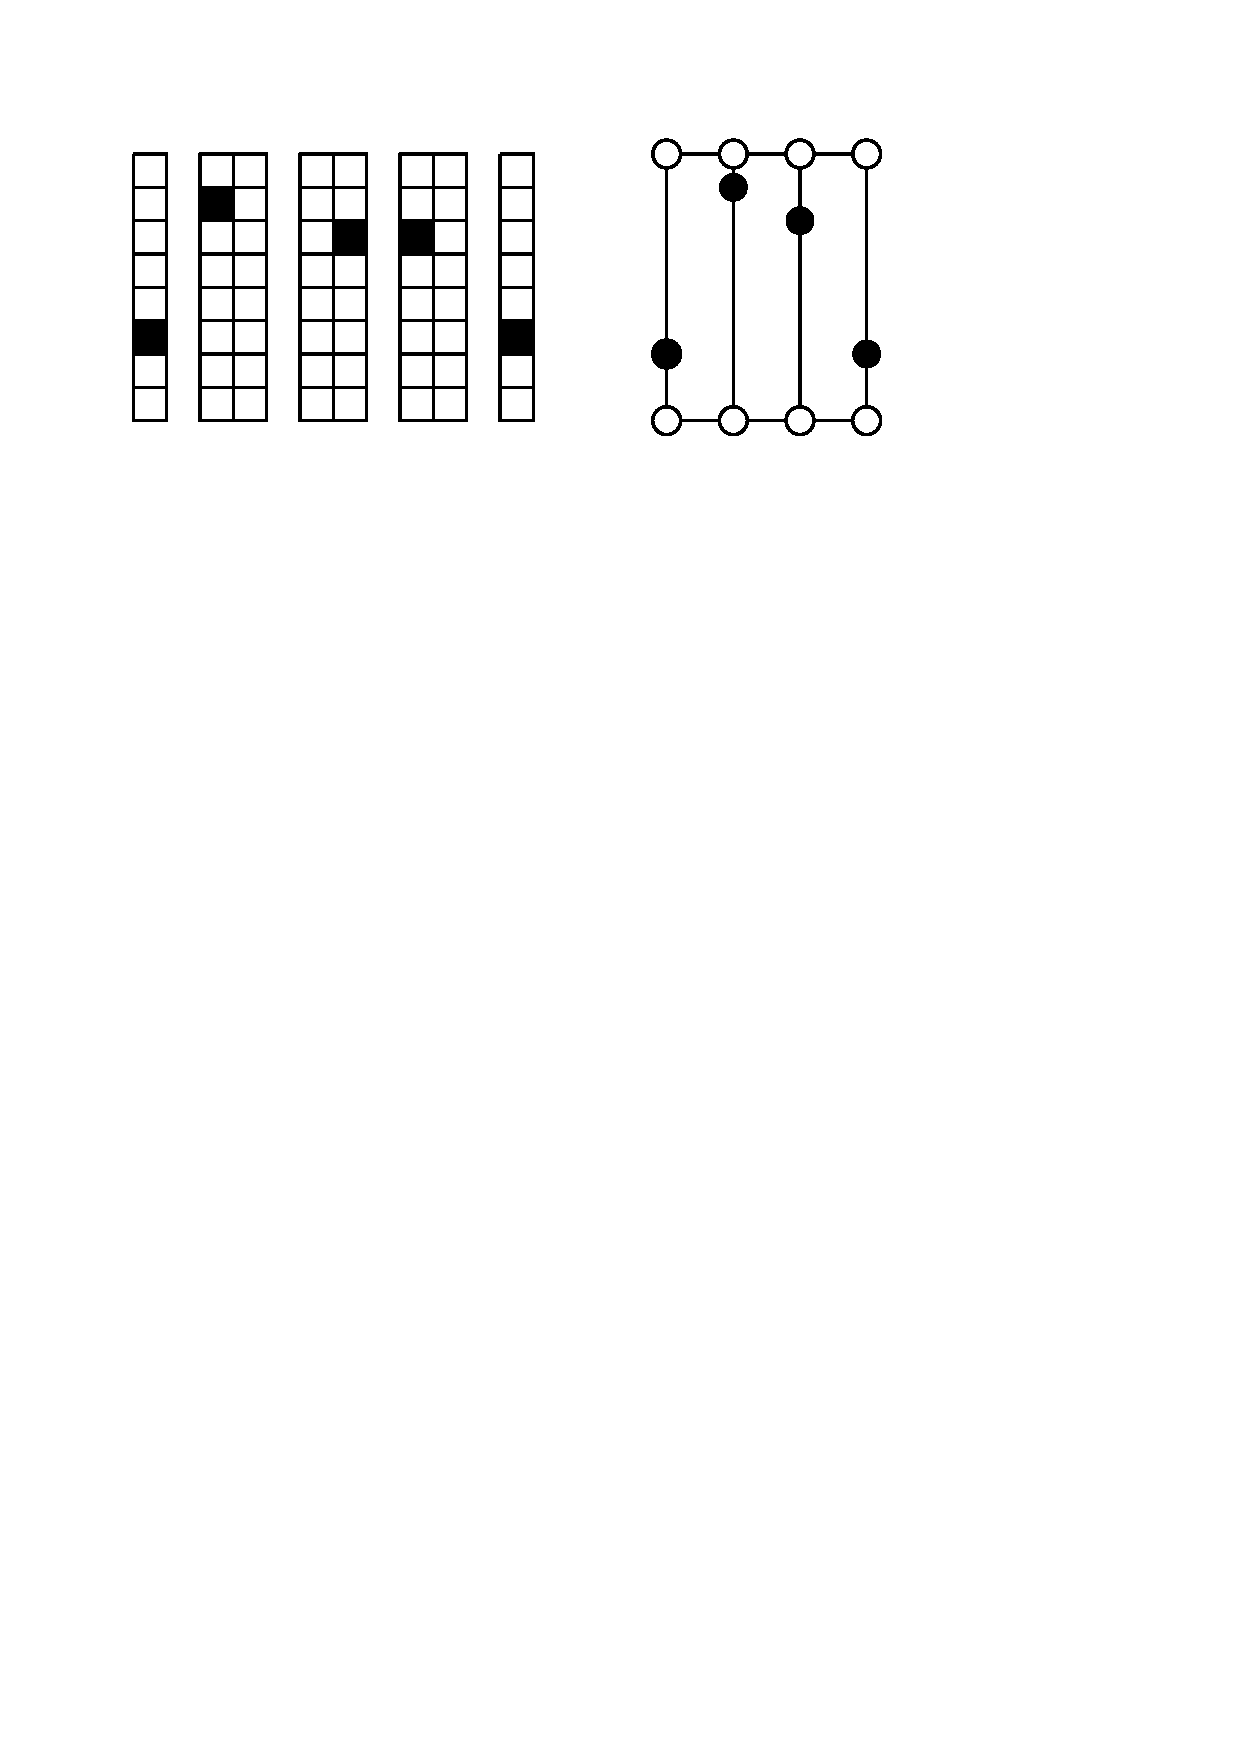
\includegraphics[width=1\linewidth]{CD_1}
			\caption{Representa\c{c}\~ao de armaz\'em via grafo}
			
		\end{figure}
	\pause
	\begin{itemize}
		\item {\bfseries Problema :}
		Infactibilidade da rota devido ao sobrevolume do palete
	\end{itemize}
	\end{frame}


%Frame dividido na tela
\begin{frame}{Descri\c{c}\~ao do problema}
	\framesubtitle{(CSPRP)}
\fboxsep=0pt
\noindent{%
	\begin{minipage}[t]{0.48\linewidth}
		\begin{itemize}
		\item[]
		\item \bfseries{Localiza\c{c}\~ao Geometrica das caixas}
		\item[] %itemize que esconde o bullet, só para o posicionamento ficar correto na imagem
		\item[]
		\item[]
		%\item \bfseries{Restri\c{c}\~oes de empilhamento m\'aximo das caixas}
		\end{itemize}

	\end{minipage}}%
\hfill%
{%
	\begin{minipage}[t]{0.48\linewidth}
		\begin{figure}			
			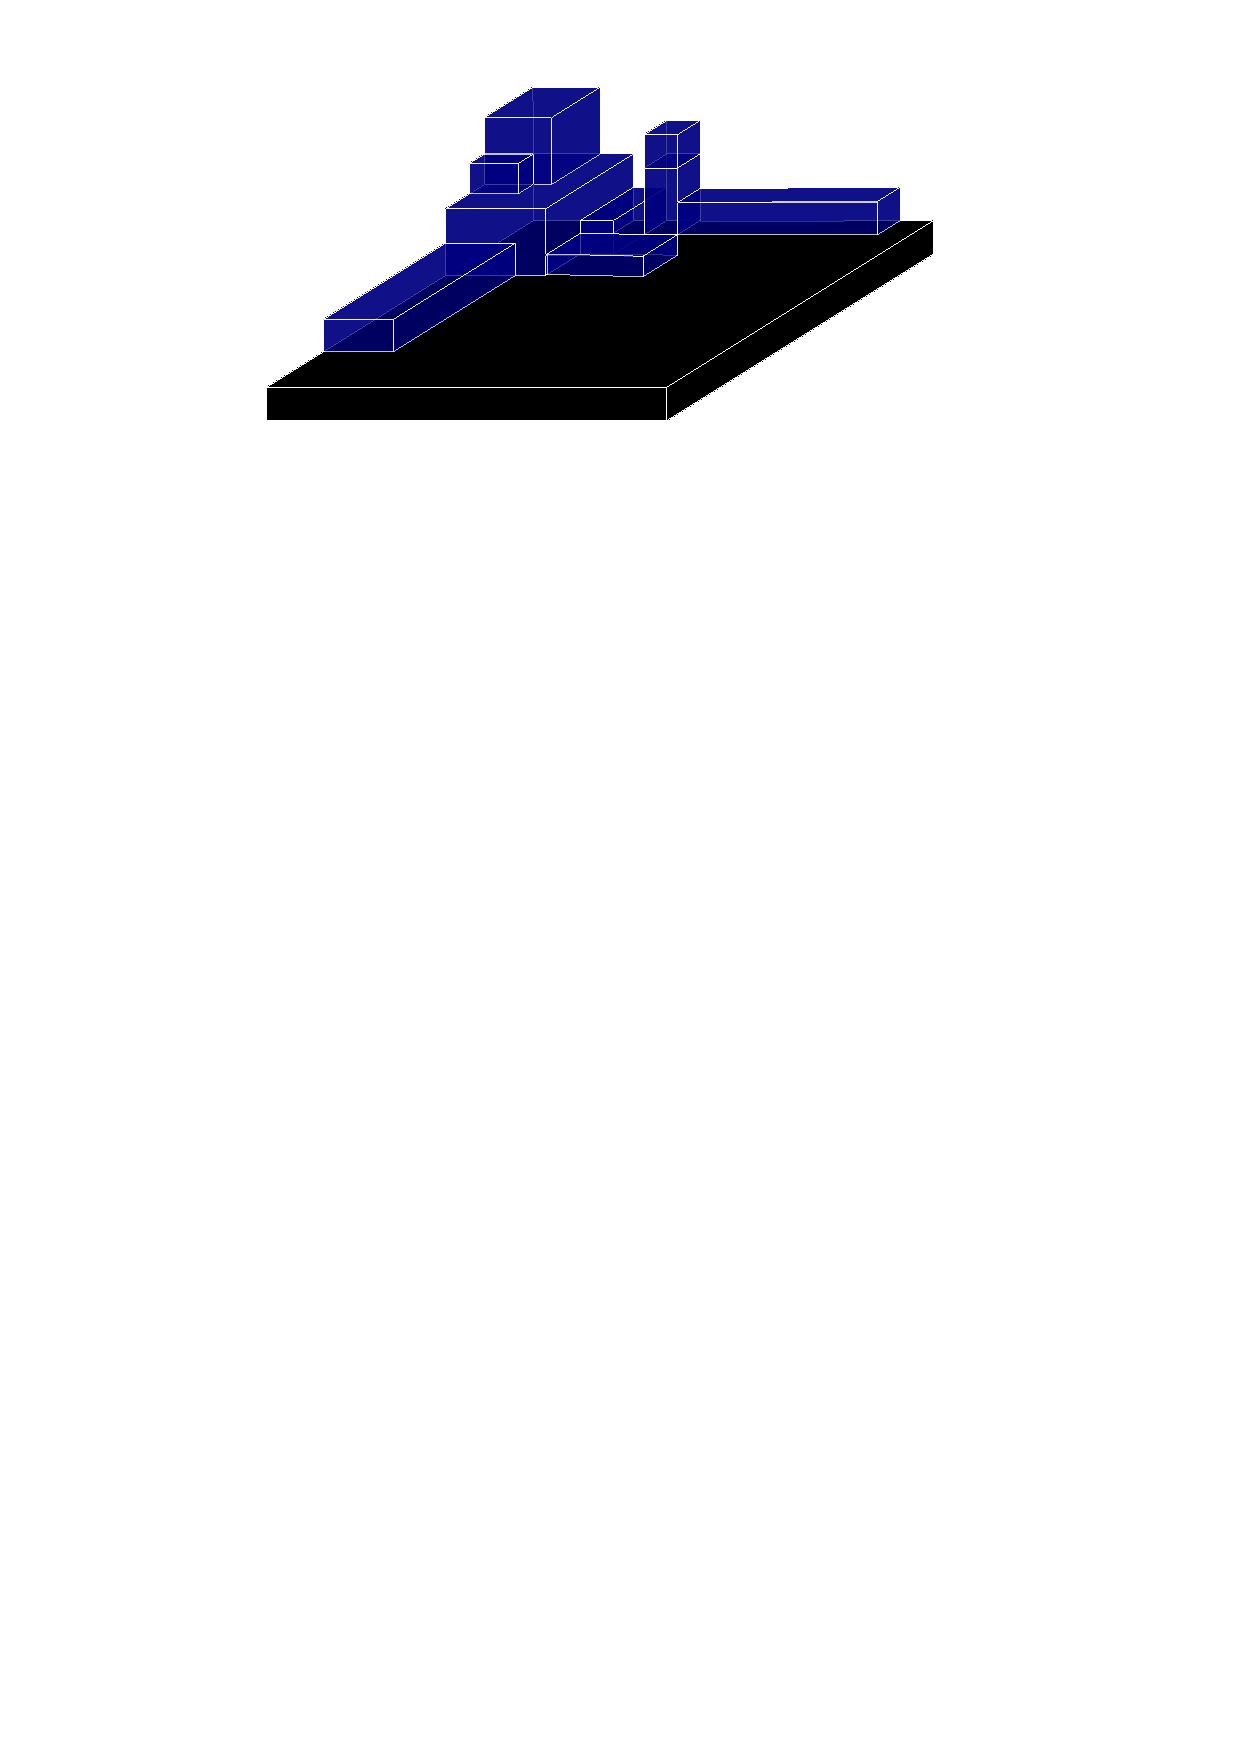
\includegraphics[width=1\linewidth]{volume_caixas}
		\end{figure}
		

	\end{minipage}
}
\end{frame}

\begin{frame}{Descri\c{c}\~ao do problema}
	\framesubtitle{(CSPRP)}
	\fboxsep=0pt
	\noindent{%
		\begin{minipage}[t]{0.48\linewidth}
			\begin{itemize}
				\item[]
				\item \bfseries{Localiza\c{c}\~ao Geometrica das caixas}
				\item[] %itemize que esconde o bullet, só para o posicionamento ficar correto na imagem
				\item[]
				\item[]
				\item \bfseries{Restri\c{c}\~oes de empilhamento m\'aximo das caixas}
			\end{itemize}
			
	\end{minipage}}%
	\hfill%
	{%
		\begin{minipage}[t]{0.48\linewidth}
			\begin{figure}			
				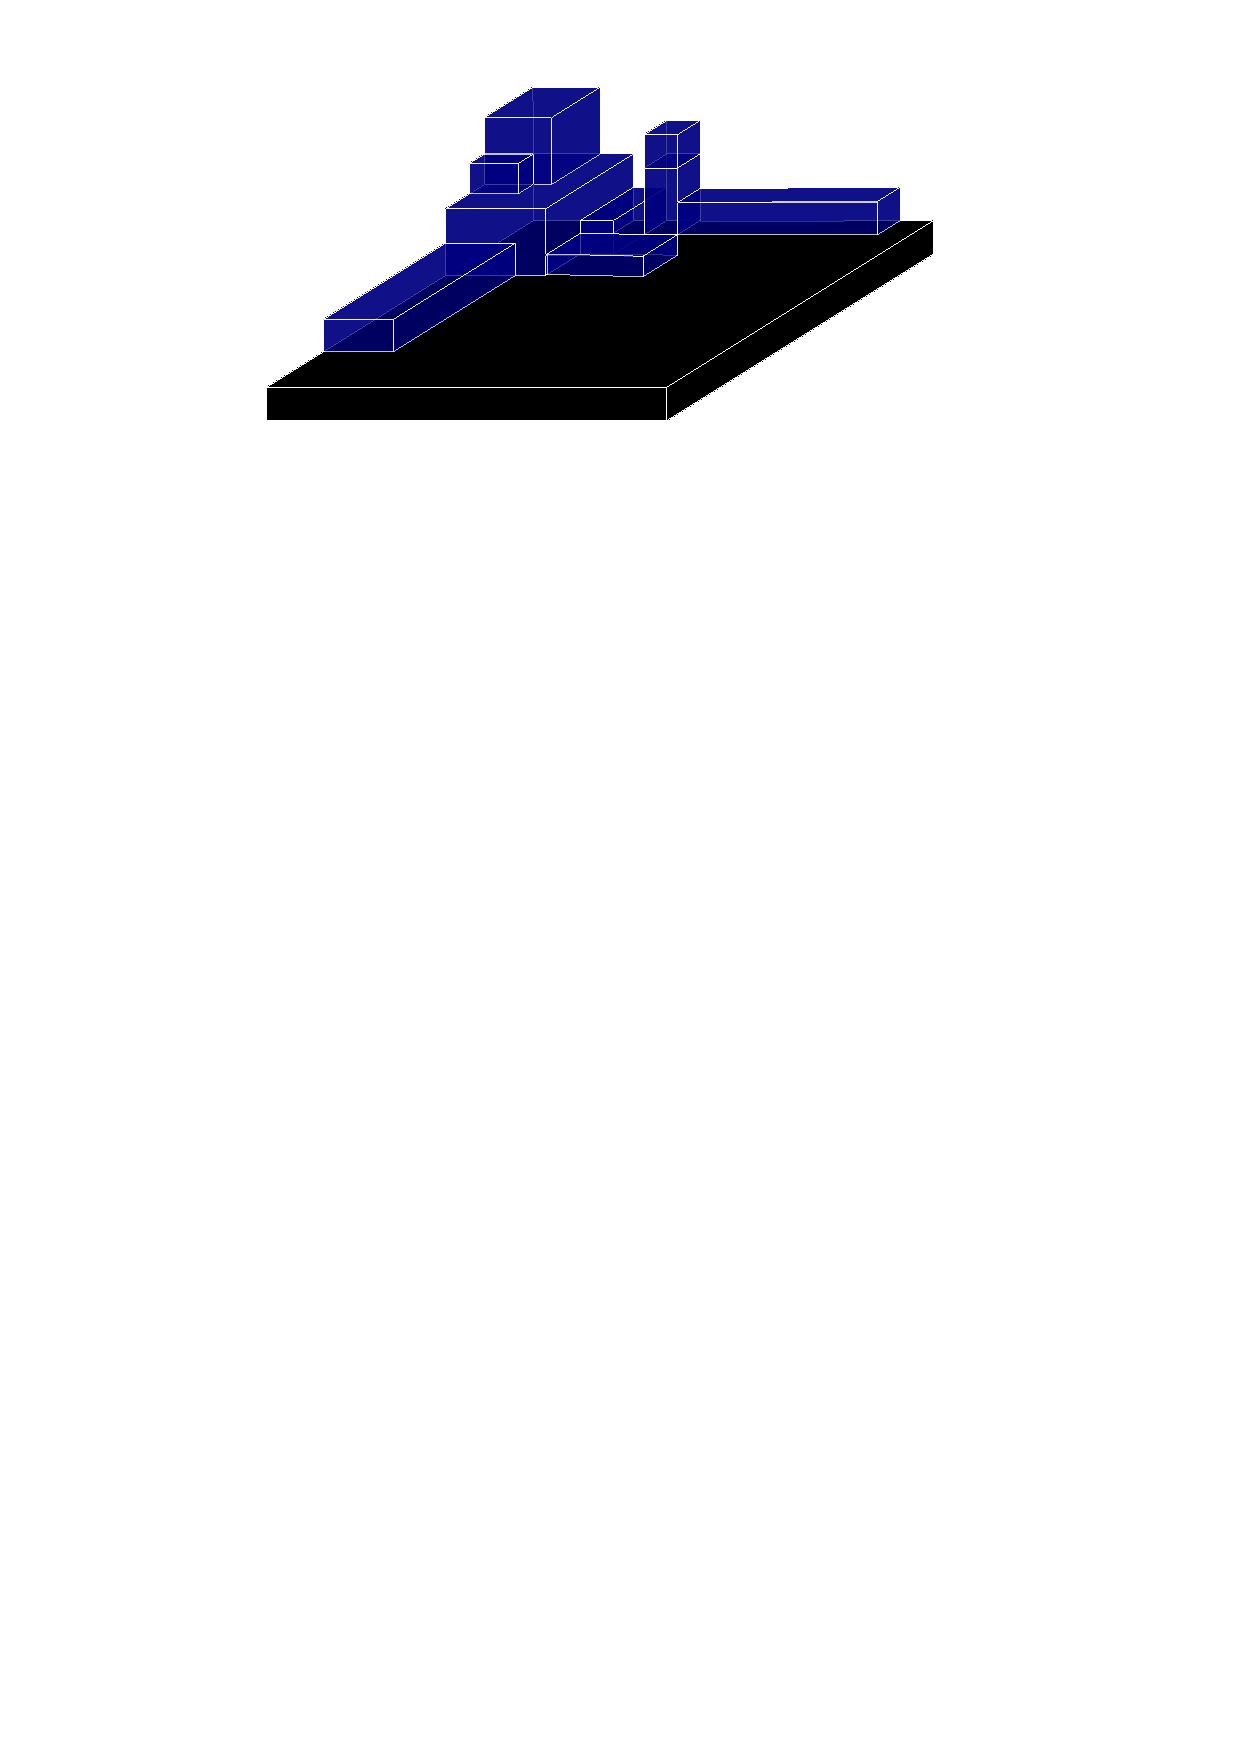
\includegraphics[width=1\linewidth]{volume_caixas}
			\end{figure}
			\begin{figure}			
				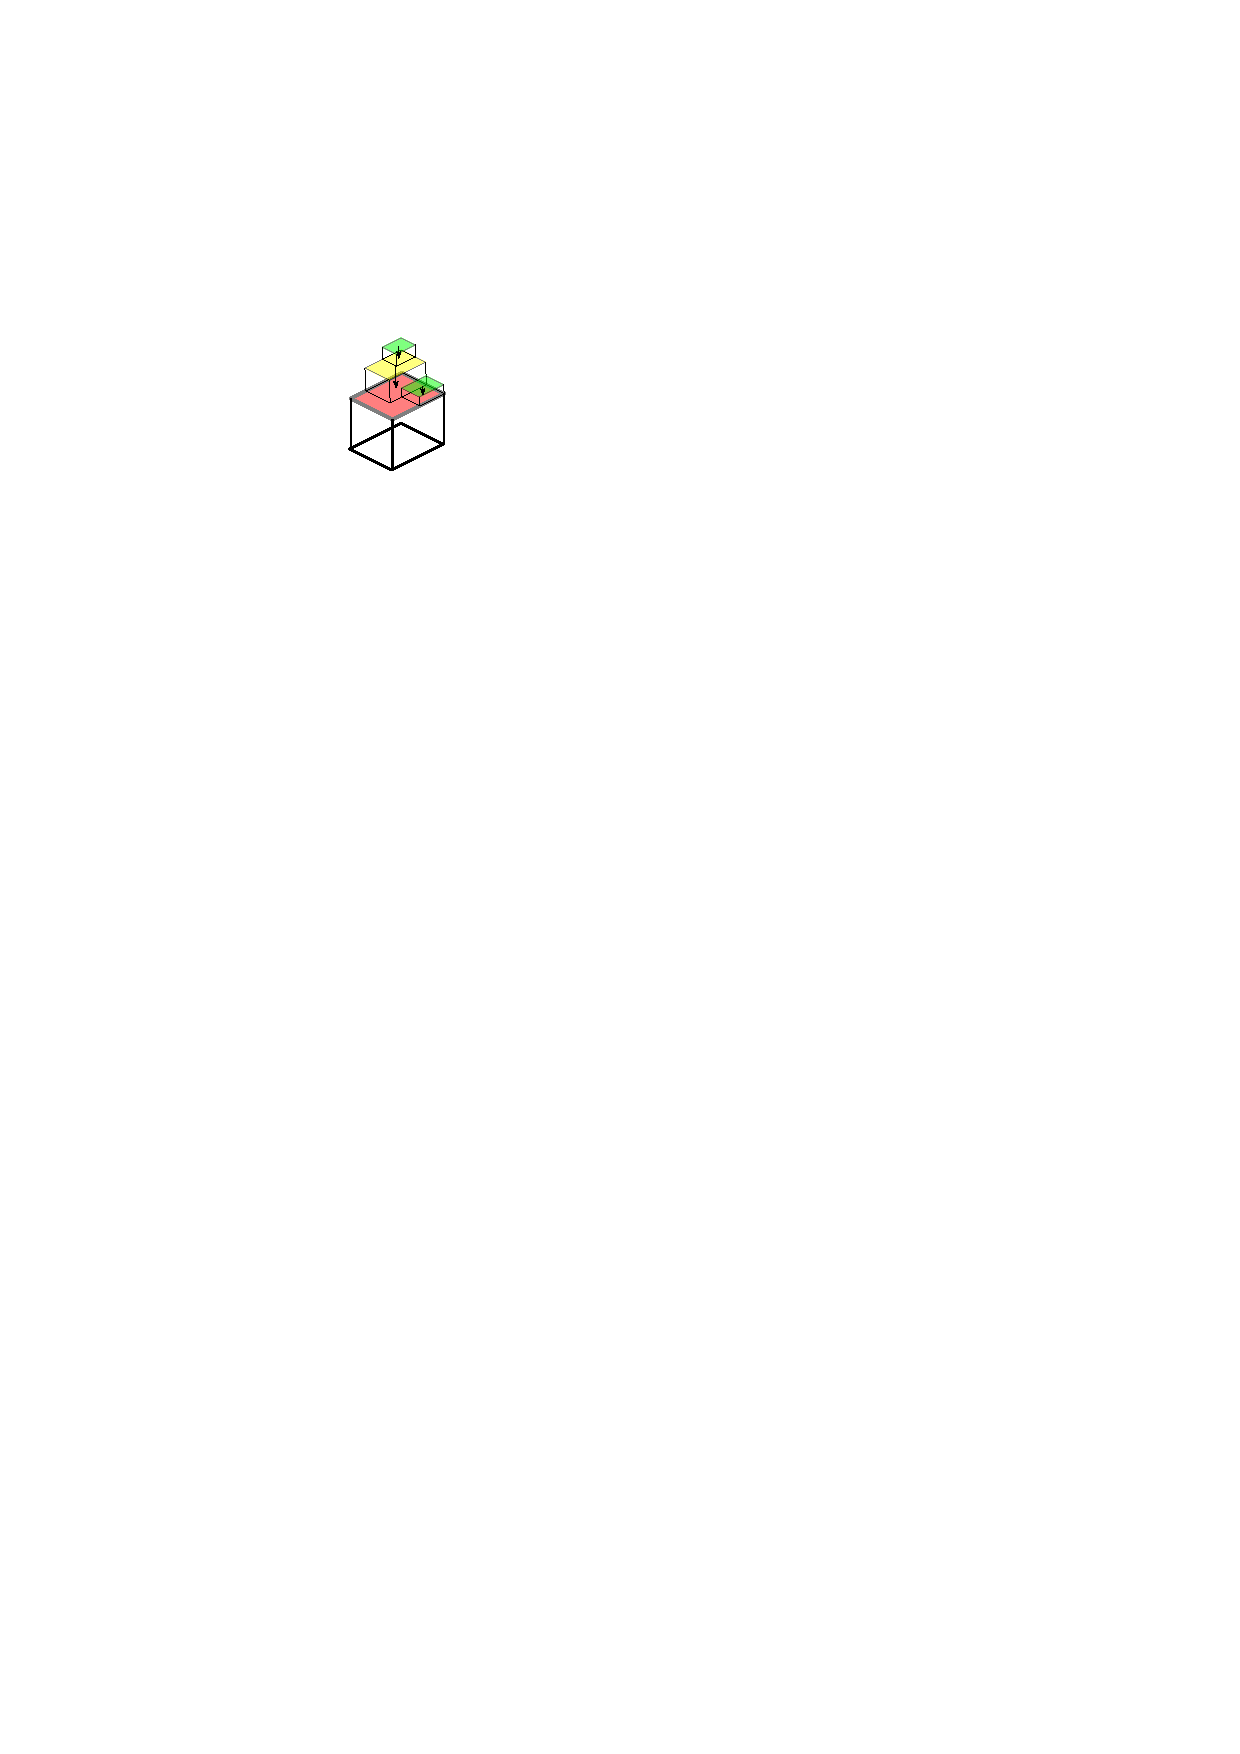
\includegraphics[width=0.45\linewidth]{pressao_caixas}
				
			\end{figure}
		\end{minipage}
	}
\end{frame}

\begin{frame}{Descri\c{c}\~ao do problema}
	\framesubtitle{(CSPRP)}
	\fboxsep=0pt
	\noindent{%
		\begin{minipage}[t]{0.48\linewidth}
			\begin{itemize}
				\item[]
				\item {{Determinar um {\bfseries conjunto}} de rotas, tais que:
					\begin{itemize}
						\item todos os itens sejam coletados 
						\item n~ao exista sobreposi\c{c}\~ao de caixas no palete 
					\end{itemize}
				 
				 
		         }
			\end{itemize}
			
	\end{minipage}}%
	\hfill%
	{%
		\begin{minipage}[t]{0.48\linewidth}
			\begin{figure}			
				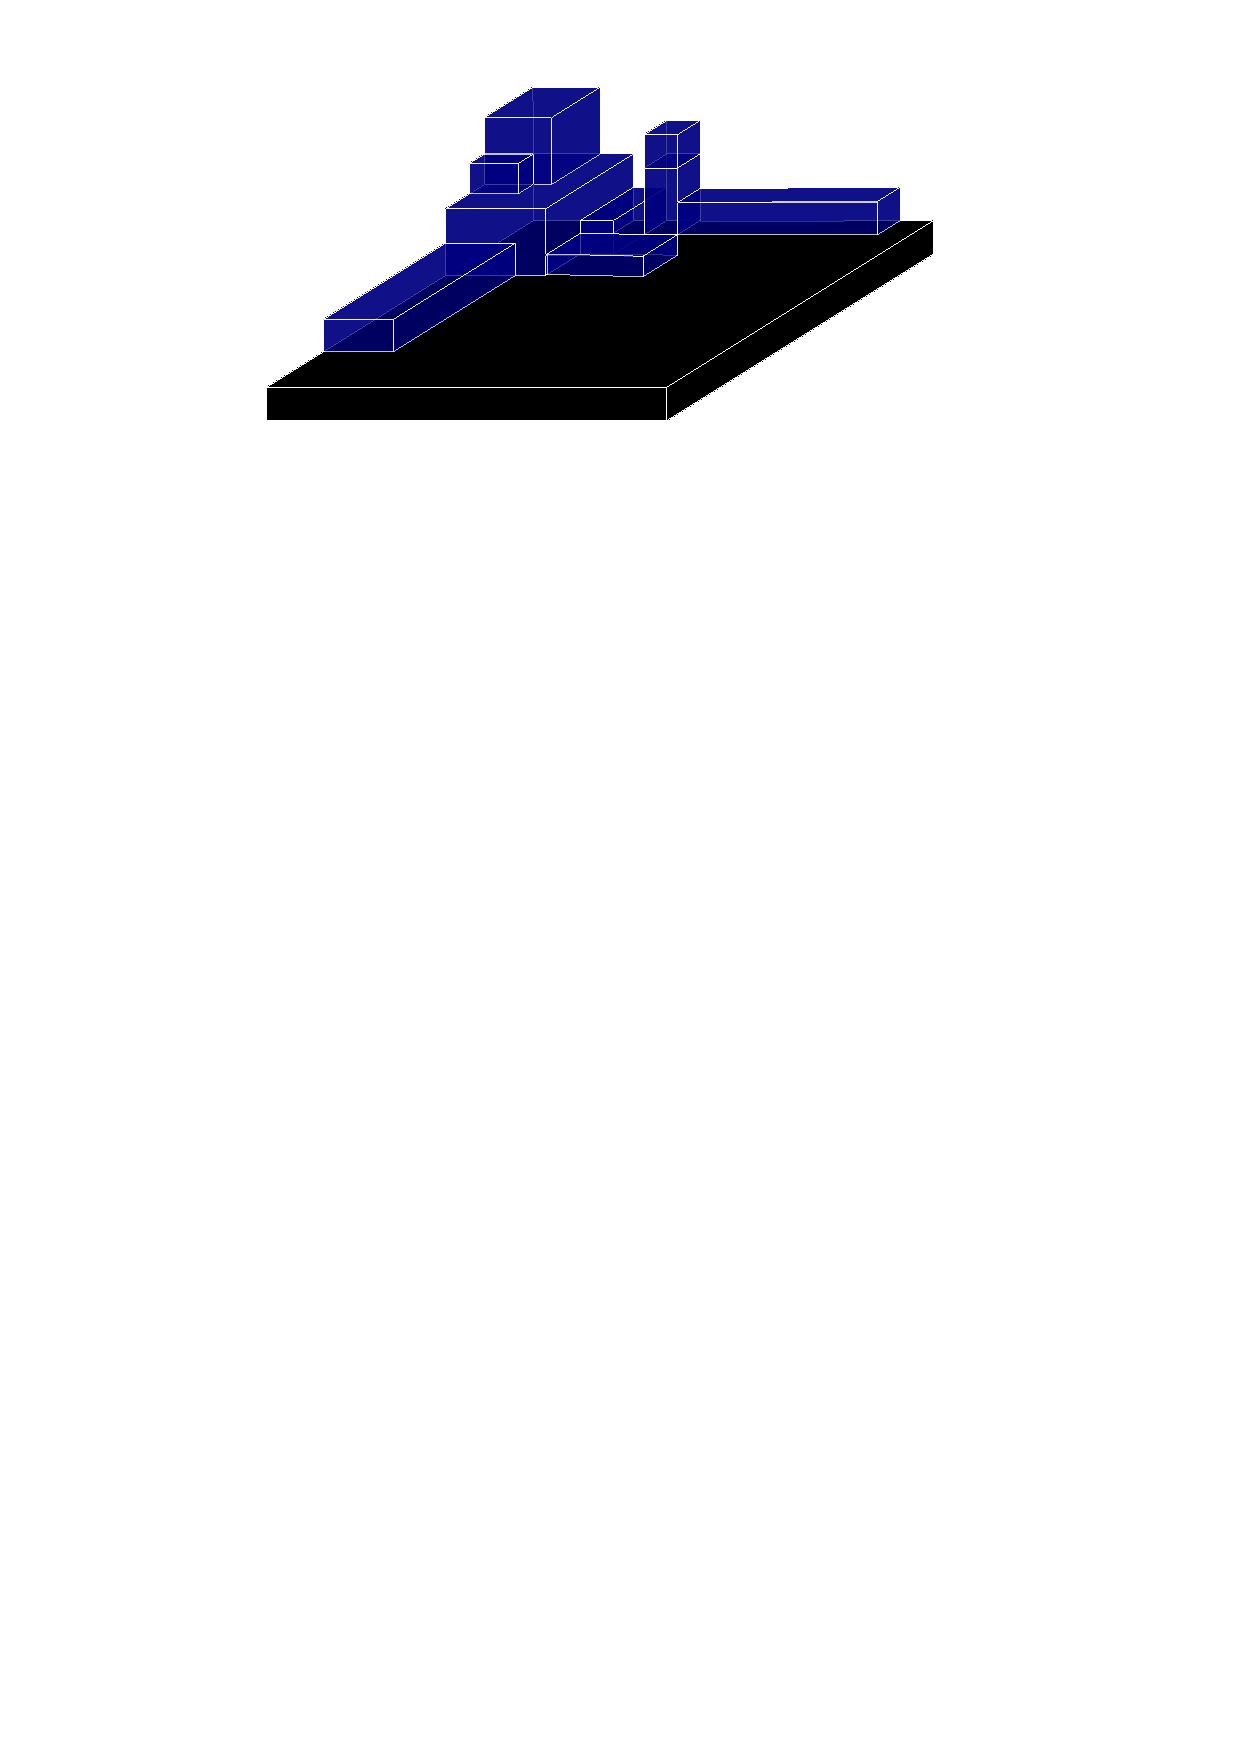
\includegraphics[width=1\linewidth]{volume_caixas}
			\end{figure}
			\begin{figure}			
				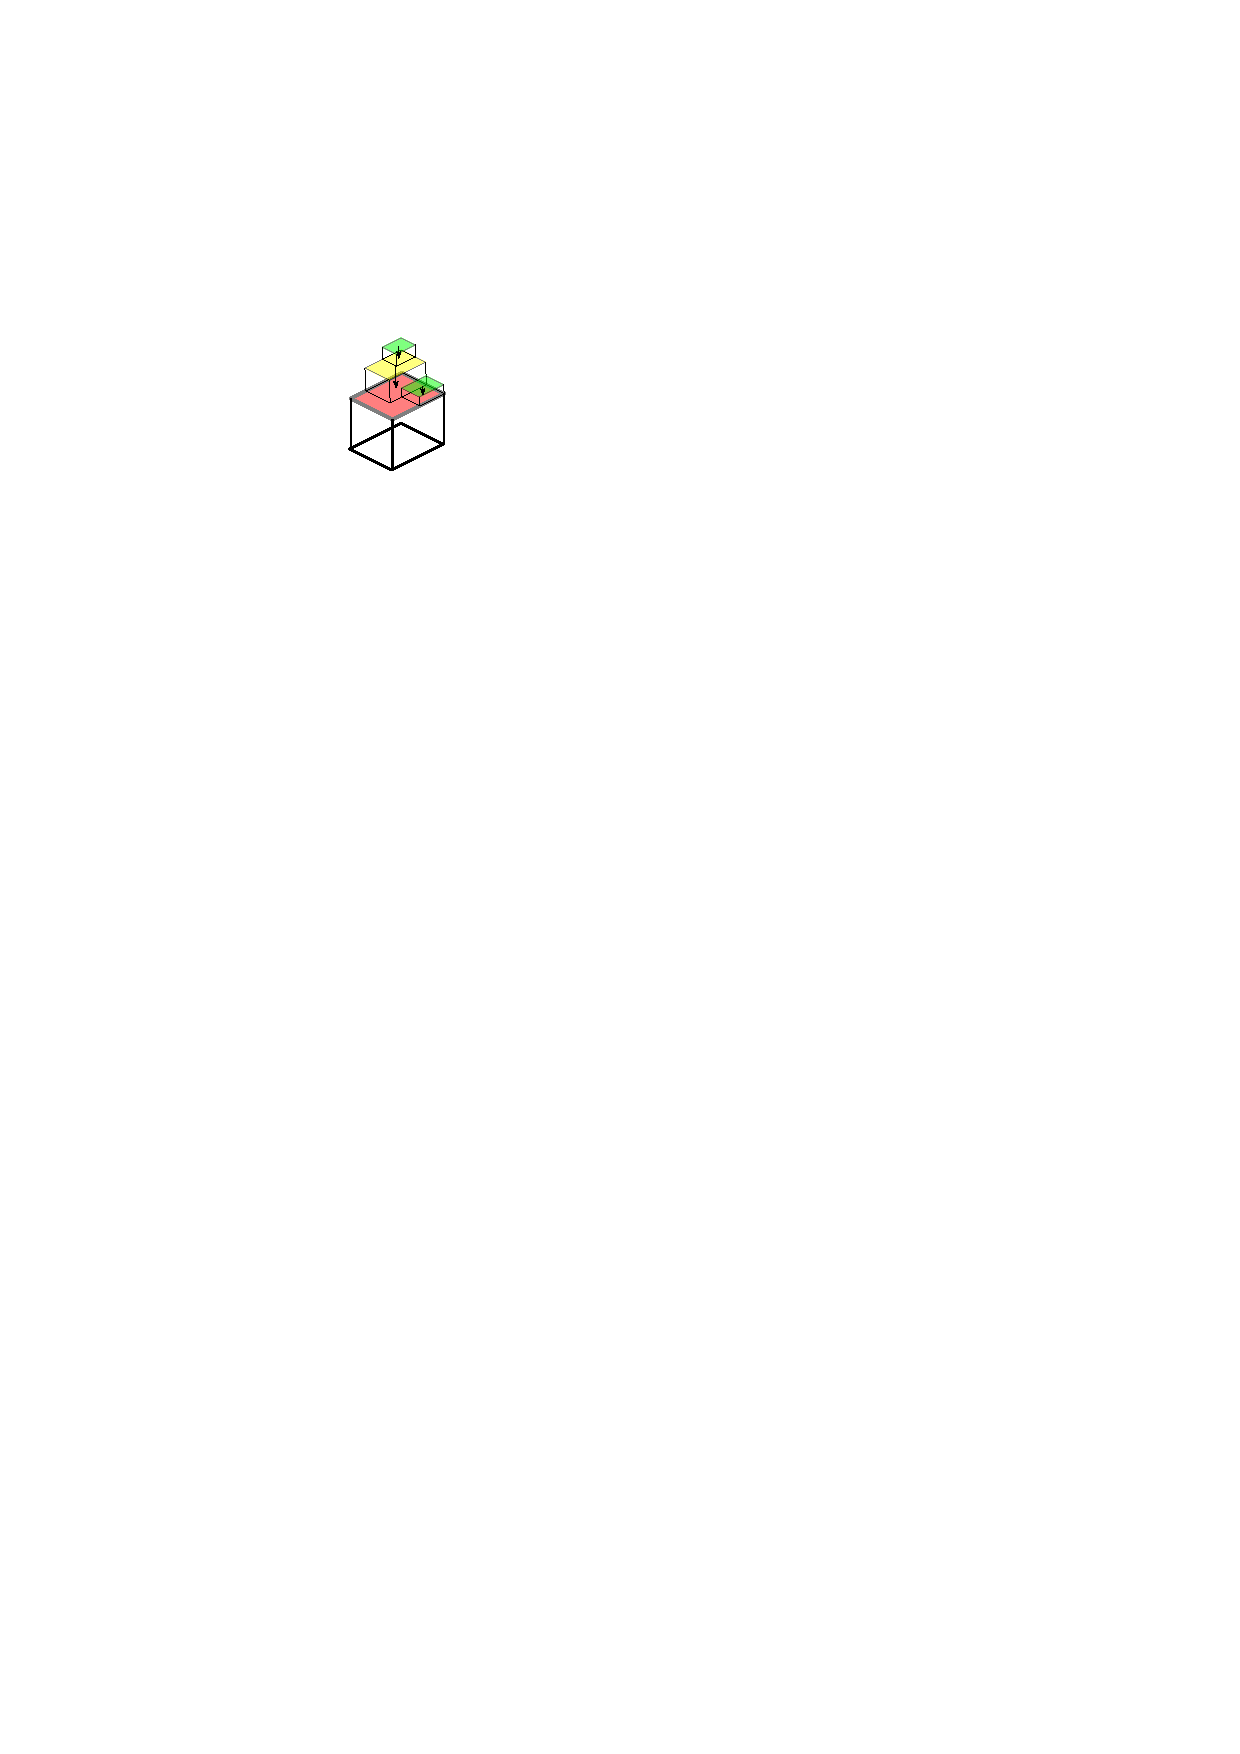
\includegraphics[width=0.45\linewidth]{pressao_caixas}
				
			\end{figure}
		\end{minipage}
	}
\end{frame}










\section{Heur\'istica de corre\c{c}\~ao de rotas} %
	\begin{frame}{Heur\'istica de corre\c{c}\~ao de rotasa}
\end{frame}
\section{Heur\'istica de Empacotamento} %
	\begin{frame}{Heur\'istica de Empacotamento}
\end{frame}
\section{Heur\'istica de Escoamento de Pontos (H.E.P)} %
	\begin{frame}{Heur\'istica de Escoamento de Pontos (H.E.P)}
\end{frame}
\section{Resultados} %
	\begin{frame}{Resultados}
\end{frame}

	
	
	
	
\end{document} 